\documentclass[ 12pt ]{article}
\usepackage{amsmath, amsthm, amssymb, enumitem, graphicx, listings, mathrsfs, tabularx}
\usepackage[margin=0.5in]{geometry}
\graphicspath{ ./ }

\begin{document}

\noindent Landon Fox \\
\noindent CS 456 \\
\noindent October 18, 2020

\begin{center}
	\Large Exam 1
\end{center}

\begin{enumerate}
	% problem 1
	\item[\textbf{1.}] Show $L = \{ a^n b^m : n + m = 2k - 1, n \geq 0, m \geq 0, k \in \mathbb{N} \}$ is regular by using
		\begin{enumerate}
			\item[\textbf{i.}] Regular expressions.
			\item[\textbf{ii.}] Regular grammars.
			\item[\textbf{iii.}] Nfas/dfas.
		\end{enumerate}

		\begin{proof}
			Suppose $\Sigma = \{ a, b \}$ and that $L = \{ a^n b^m : n + m = 2k - 1, n \geq 0, m \geq 0, k \in \mathbb{N} \}$.
			\begin{enumerate}
				\item[\textbf{i.}] Let $r = (aa)^*(a + b)(bb)^*$. Clearly we can see that $r$ is a regular expression; by Definition 3.1, $r$ is derived from the primitive regular
					expressions $a$ and $b$ by applying well defined operations upon them that guarantee closure. \\ \\
					Now, I claim that $L = L(r)$. For any string $w \in L$ we can see that $n_a(w)$ and $n_b(w)$ must have opposite parity and so either $n_a(w)$ or $n_b(w)$ is odd but
					not both. Turning our attention to $L(r)$, any string $w$ belonging to it must begin with an arbitrary even number of $a$'s and end with an arbitrary even number of
					$b$'s with the addition of either an $a$ or $b$ in the middle, but not both, ensuring that either $n_a(w)$ or $n_b(w)$ is odd but not both. Then it follows that all
					strings in $L$ and $L(r)$ share the same properties, hence any string $w \in L$ implies that $w \in L(r)$ and any string $w \in L(r)$ implies that $w \in L$; therefore,
					$L \subseteq L(r)$ and $L(r) \subseteq L$, and so $L = L(r)$ as claimed. \\ \\
					Provided that $r$ is a regular expression and that $r$ describes the language $L$, Theorem 3.1 states that $L$ must be regular.

				\item[\textbf{ii.}] Consider the grammar $G = (\{ S, A, B \}, \Sigma, S, P)$ where $P$ is defined as the set of productions
					\begin{align*}
						S &\to aaS | A \\
						A &\to aB | bB \\
						B &\to bbB | \lambda.
					\end{align*}
					Clearly we can see that $G$ is a regular grammar becuase it is a right-linear grammar. \\ \\
					Let us now show that $L = L(G)$. Beginning with production $S$, you can repeatedly choose an even number of $a$'s and then you must continue to $A$. From $A$, you can
					either take an $a$ or $b$ then continue to $B$ where you can take an even number of $b$'s and terminate the production of the string via $\lambda$. Moreover, any
					string in $L(G)$ must begin with with an even number of $a$'s and end with an even number of $b$'s where you are forced to take a single $a$ or $b$ in the middle.
					We can then see that for a string $w \in L(G)$ has the property that $n_a(w)$ and $n_b(w)$ have different parities. The properties of $L$, as depicted in \textbf{1i},
					are shared by $L(G)$; hence, any string $w \in L$ implies that $w \in L(G)$ and any string $w \in L(G)$ implies that $w \in L$; therefore, $L \subseteq L(G)$ and
					$L(G) \subseteq L$, and so $L = L(G)$ as claimed. \\ \\
					Provided that $G$ is a regular grammar and that $G$ describes the language $L$, Theorem 3.3 states that $L$ must be regular.

				\item[\textbf{iii.}] Let $M = ( \{ q_i : i = 0, 1, \hdots, 7 \}, \Sigma, \delta, q_0, \{ q_7 \})$ be an nfa. I claim that $L = L(M)$. Clearly any accepted string
					in $L(M)$ must start from $q_0$ and reach $q_2$ as well as $q_5$ on the path to $q_7$. Any path from $q_0$ to $q_2$ must accumulate an even number of $a$'s, or rather
					$q_2 \in \delta^*(q_0, a^{2k})$ for any $k \in \mathbb{N} \cup \{ 0 \}$. Similarly, any path from $q_5$ to $q_7$ must accumulate an even number of $b$'s, or rather
					$q_7 \in \delta^*(q_5, b^{2k})$ for any $k \in \mathbb{N} \cup \{ 0 \}$. Unlike the other two paths, the paths from $q_2$ to $q_5$ provide either a single $a$ or $b$,
					but not both. Furthermore, any string $w \in L(M)$ must have the property that $n_a(w)$ and $n_b(w)$ have different parities. The properties of $L$, as depicted in
					\textbf{1i}, are shared by as $L(M)$; hence, any string $w \in L$ implies that $w \in L(M)$ and any string $w \in L(M)$ implies that $w \in L$; therefore, $L
					\subseteq L(M)$ and $L(M) \subseteq L$, and so $L = L(M)$ as claimed. \\ \\
					Provided that $M$ is a nfa and that $M$ describes the language $L$, $L$ is regular by definition since there is an equivalence between nfas and dfas.
			\end{enumerate}
		\end{proof}


	% problem 2
	\item[\textbf{2.}] Convert the following nfa to an equivalent dfa. 
		\begin{center}
			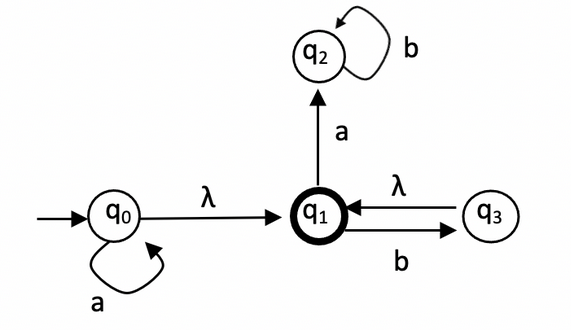
\includegraphics{Capture}
		\end{center}

		\begin{proof}[Solution]
			Observe that
			\begin{center}
			\begin{tabularx}{0.5\textwidth}{
				>{\raggedright\arraybackslash}X
				>{\raggedright\arraybackslash}X }
				$\delta^* \left( \{ q_0 \}, a \right) = \{ q_0, q_1, q_2 \}$ & $\delta^* \left( \{ q_0 \}, b \right) = \{ q_1, q_3 \}$ \\
				$\delta^* \left( \{ q_1 \}, a \right) = \{ q_2 \}$ & $\delta^* \left( \{ q_1 \}, b \right) = \{ q_1, q_3 \}$ \\
				$\delta^* \left( \{ q_2 \}, a \right) = \emptyset$ & $\delta^* \left( \{ q_2 \}, b \right) = \{ q_2 \}$ \\
				$\delta^* \left( \{ q_3 \}, a \right) = \{ q_2 \}$ & $\delta^* \left( \{ q_3 \}, b \right) = \{ q_3 \}$.
			\end{tabularx}
			\end{center}
			Now considering the newly added states $\{ q_1, q_3 \}$, $\{ q_0, q_1, q_2 \}$, and $\emptyset$, we have
			\begin{center}
			\begin{tabularx}{1\textwidth}{
				>{\raggedright\arraybackslash}X
				>{\raggedright\arraybackslash}X }
				$\delta^* \left( \{ q_1, q_3 \}, a \right) = \{ q_2 \} \cup \{ q_2 \} = \{ q_2 \}$ & $\delta^* \left( \{ q_1, q_3 \}, b \right) = \{ q_1, q_3 \} \cup \{ q_3 \} = \{ q_1, q_3 \}$ \\
				$\delta^* \left( \{ q_0, q_1, q_2 \}, a \right) = \{ q_0, q_1, q_2 \} \cup \{ q_2 \} \cup \emptyset = \{ q_0, q_1, q_2 \}$ & $\delta^* \left( \{ q_0, q_1, q_2 \}, b \right) = \{ q_1, q_3 \} \cup \{ q_1, q_3 \} \cup \{ q_2 \} = \{ q_1, q_2, q_3 \}$ \\
				$\delta^* \left( \emptyset, a \right) = \emptyset$ & $\delta^* \left( \emptyset, b \right) = \emptyset$.
			\end{tabularx}
			\end{center}
			Again, with the new state $\{ q_1, q_2, q_3 \}$, we obtain
			\begin{center}
			\begin{tabularx}{1\textwidth}{
				>{\raggedright\arraybackslash}X
				>{\raggedright\arraybackslash}X }
				$\delta^* \left( \{ q_1, q_2, q_3 \}, a \right) = \{ q_2 \} \cup \emptyset = \{ q_2 \}$ & $\delta^* \left( \{ q_1, q_2, q_3 \}, b \right) = \{ q_1, q_3 \} \cup \{ q_2\} = \{ q_1, q_2, q_3 \}$.
			\end{tabularx}
			\end{center}
			Since $\lambda$ is accepted by our nfa and $q_1$, the final state of the nfa, is included in many of our states, we can then see that our dfa is
			\begin{align*}
				M_d = (\;& \\
				&\{ \emptyset, \{q_0\}, \{q_2\}, \{q_1, q_3\}, \{q_0, q_1, q_2\}, \{q_1, q_2, q_3\} \}, \\
				&\{ a, b \}, \\
				&\delta_d, \\
				&\{ q_0 \}, \\
				&\{ \{q_0\}, \{q_1, q_3\}, \{q_0, q_1, q_2\}, \{q_1, q_2, q_3\} \} \\
				).\;&
			\end{align*}
		\end{proof}


	% problem 3
	\item[\textbf{3.}] Using nfas/dfas prove that regular languages are closed under the concatenation operation.

		\begin{proof}
			Suppose $L_1$ and $L_2$ are regular languages. Then by definition there must exist nfas $M_1 = (Q, \Sigma, \delta_1, q_0, F_1)$ and $M_2 = (P, \Gamma, \delta_2, p_0, F_2)$
			since nfas and dfas are equivalent. Without loss of generality, let the languages be concatenated as $L_1 L_2$ (rather than $L_2 L_1$). Further, let $M_3 = (Q \cup P,
			\Sigma \cup \Gamma, \delta_3, q_0, F_2)$ where $\delta_3 : (Q \cup P) \times (\Sigma \cup \Gamma \cup \{ \lambda \}) \to 2^{Q \cup P}$ is defined as
			\begin{itemize}
				\item $\delta_3(q, \sigma) = \delta_1(q, \sigma)$ for all $q \in Q$ and $\sigma \in \Sigma \cup \{ \lambda \}$.
				\item $\delta_3(p, \gamma) = \delta_2(p, \gamma)$ for all $p \in P$ and $\gamma \in \Gamma \cup \{ \lambda \}$.
				\item $\delta_3(f, \lambda) = p_0$ for all $f \in F_1$.
			\end{itemize}
			In other words, $\delta_3$ takes the value of both $\delta_1$ and $\delta_2$ and appends the two nfas by providing the final states of $M_1$ a $\lambda$ transition to
			the initial state of $M_2$. \\ \\
			I claim that $L_1 L_2 = L(M_3)$.
			Suppose a string $w \in L_1 L_2$, then by definition of concatenation, $w = uv$ where $u \in L_1$ and $v \in L_2$. By our definition of $\delta_3$, it follows that
			$\delta_3^*(q_0, u) = F_1 \cup \{ p_0 \}$; likewise, it must hold that $\delta_3^*(p_0, v) = F_2$. Therefore, $\delta_3^*(q_0, uv) = F_2$ implying that $w= uv$ is accepted
			by $M_3$, hence $L_1 L_2 \subseteq L(M_3)$. Now consider another string $w \in L(M_3)$. Similarly, we know that $w$ can be decomposed into two concatenated strings, one
			that reaches a final state of $M_1$ and one that can reach the final state of $M_2$ starting from $p_0$ which illustrates that $w \in L_1 L_2$ and so $L(M_3) \subseteq
			L_1 L_2$. Furthermore, $L_1 L_2 = L(M_3)$ as claimed. Since $M_3$ is an nfa by definition, it must follow that $L_1 L_2$ is also regular, again by the equivance of nfas and
			dfas.
		\end{proof}


	% problem 4
	\item[\textbf{4.}] Using the pumping lemma show that $L = \{ a^{n!} : n \in \mathbb{N} \}$ is not regular.

		\begin{proof}
			Let us first recall the definition of the pumping lemma. An extention of the pigeonhole principle, the pumping lemma for infinite regular languages, states that for any
			infinite regular language $L$, there exists a $p \in \mathbb{N}$ (labeled the pumping length) such that for any string $w \in L$ with $|w| \geq p$ then $w = xyz$ where $|xy|
			\leq p$ and $|y| \geq 1$ such that $w_k = xy^kz$ is also a member of $L$ for all $k \in \mathbb{N} \cup \{ 0 \}$. \\ \\
			Suppose $\Sigma = \{ a \}$ and that $L = \{ a^{n!} : n \in \mathbb{N} \}$. Further, by contradiction suppose $L$ is a regular language. Clearly $L$ is an infinite language
			and regular by assumption, then by the pumping lemma there must exist a pumping length $p \in \mathbb{N}$ for any string in our language where its length exceeds $p-1$.
			Let $w = a^{(p+2)!} \in L$ where $|w| = (p+2)! \geq p$. The pumping lemma also states that our string can be decomposed to $w = xyz$ where $y = a^k$ for $1 \leq k \leq p$
			since $|xy| \leq p$ and $|y| \geq 1$. Let us pump $w = a^{p - k} a^k a^{(p+2)! - p}$ down to $w_0 = a^{p - k} a^{(p+2)! - p} = a^{(p+2)! - k}$. Now, observe that $n_a(w_0) =
			(p+2)! - k$ implies that $$(p+1)! = (p+2)! - (p+1)(p+1)! \leq (p+2)! - p \leq n_a(w_0) \leq (p+2)! - 1 < (p+2)!.$$ Since $n!$ is a strictly increasing function on $\mathbb{N}$
			and $w_0 \in L$ by assumption, $n_a(w_0) = (p+2)! - k = (p+1)!$ must hold becuase no other value of $n!$ can lie between $(p+1)!$ and $(p+2)!$; moreover, $k = (p+2)! - (p+1)!
			= (p+1)(p+1)!$. Due to the constraint $1 \leq k \leq p$, we can see that $k = (p+1)(p+1)! \leq p$ which yields $(p+1)^2(p-1)! \leq 1$ because $p | (p+1)!$. For all $n \in
			\mathbb{N}$ both $(n+1)^2 > 1$ and $(n-1)! \geq 1$ illustrating that $(p+1)^2(p-1)! \leq 1$ is a contradiction and so $L$ is not regular.
		\end{proof}


	% problem 5
	\item[\textbf{5.}] To show that $L = \{ a^n b^m : n \neq m, n \geq 0, m \geq 0 \}$ is not regular, a representative string $s = a^{p!} b^{(p+1)!}$ could be used. Explain why $s$
		is a \textit{good} string to use.

		\begin{proof}
			Let us first show that $L =  \{ a^n b^m : n \neq m, n \geq 0, m \geq 0 \}$ is not regular via the use of the pumping lemma and $s = a^{p!} b^{(p+1)!}$. Recall the definition
			of the pumping lemma as stated in \textbf{4}. \\ \\
			Suppose $\Sigma = \{ a, b \}$. Further, by contradiction suppose $L$ is a regular language. Clearly $L$ is an infinite language and regular by assumption, then by the pumping
			lemma there must exist a pumping length $p \in \mathbb{N}$ for every string in our language where its length exceeds $p-1$. Now examining $s$ where $|s| = p! + (p+1)! \geq p$,
			the pumping lemma states that our string can be decomposed to $s = xyz$ where $y = a^k$ for $1 \leq k \leq p$ since $|xy| \leq p$ and $|y| \geq 1$. Let us pump
			$s = a^{p! - k} a^k b^{(p+1)!}$ to $s_i = a^{p! - k} a^{ki} b^{(p+1)!}$ where $i = \frac{p \cdot p!}{k} + 1$. Observe that $i$ is clearly a positive value; additionally,
			$k | p!$ which implies that $i \in \mathbb{N}$ and so the pumping is valid. However, notice that $$n_a(s_0) = p! - k + ki = p! - k + k \left ( \frac{p \cdot p!}{k} + 1
			\right ) = p! + p \cdot p! = (p+1)! = n_b(s_0)$$ which is a contradiction. Thus, $L$ is not a regular language. \\ \\
			The string $s$ is a good choice for primarily one reason, the existence of $i \in \mathbb{N} \cup \{ 0 \}$ which satisfies the equation $p! - k + ki = (p+1)!$. For our
			specific language, we desire to select a string $s$ so that there exists an $i$ such that $n_a(s_i) = n_b(s_i)$ so that $s_i \notin L$ proving the claim. Selecting
			a string as we normally would provides some difficulty; moreover, by choosing $s = a^{p!} b^{(p+1)!}$, our $y = a^k$ for any value of $1 \leq k \leq p$ due to the constraints
			of the pumping lemma (as seen above). Then, by pumping $s$ to $s_i = a^{p! - k} a^{ki} b^{(p+1)!}$ we have $n_a(s_i) = p! - k + ki$ and $n_b(s_i) = (p+1)!$. As illustrated
			above, there does in fact exist an $i = \frac{p \cdot p!}{k} + 1 \in \mathbb{N} \cup \{ 0 \}$ such that $n_a(s_i) = n_b(s_i)$ which makes this choice desirable.
		\end{proof}
\end{enumerate}

\end{document}
